\subsubsection{Initial Value (updated to assemble right to left like the other gadgets)}
    We begin by encoding $\mathcal{C}_0$ with the Seed unit. It has $\ceil*{\frac{d}{3}}$ digit regions.
    Each digit region has three digits, except for the most significant digit region (MSR) which has $d \mod 3$
    if $d \mod 3 \not= 0$, otherwise it has 3 digits.


while $i < d$:

\begin{itemize}
    \item if $i = 0$: create
    $\begin{aligned}[t]
        {\tt SeedStart}(&\left\langle {\tt SeedDigit1}, i \right\rangle \; )
    \end{aligned}$

    \item {\tt Digit1} - for each $j=0,\ldots,l$ and each $b$ in $bin(C_0[i])[j]$:
    \begin{itemize}
        \item if $j = 0$: create
        $\begin{aligned}[t]
            \dwriter(&\left\langle {\tt SeedDigit1}, i \right\rangle, \left\langle {\tt SeedBit}, i, j + 1 \right\rangle \;)
        \end{aligned}$ from the general gadget shown in Figure~\ref{fig:write_0} if $b = 0$ or Figure~\ref{fig:write_1} if $b = 1$.

        \item if $0 \leqslant j \leqslant l$: create
        $\begin{aligned}[t]
            \dwriter(&\left\langle {\tt SeedBit}, i, j \right\rangle, \left\langle {\tt SeedBit}, i, j + 1 \right\rangle \;)
        \end{aligned}$ from the general gadget shown in Figure~\ref{fig:write_0} if $b = 0$ or Figure~\ref{fig:write_1} if $b = 1$.

        \item if $j = l$:
        $\begin{aligned}[t]
            \dwriter(&\left\langle {\tt SeedBit}, i, j \right\rangle, \left\langle {\tt SeedDigitTop}, i \right\rangle \;)
        \end{aligned}$ from the general gadget shown in Figure~\ref{fig:write_0} if $b = 0$ or Figure~\ref{fig:write_1} if $b = 1$.
    \end{itemize}


    \item {\dtop}: the following statements create the gadget shown in Figure~\ref{fig:digit_top_general}
    \begin{itemize}
        \item Create
        $\begin{aligned}[t]
            {\tt North\_Line5}(& \left \langle {\tt SeedDigitTop},  i \right\rangle,
                                 \left \langle {\tt SeedDigitTopA}, i \right\rangle \;)
        \end{aligned}$ from the micro-gadget\\shown in Figure~\ref{fig:north_line}

        \item Create
        $\begin{aligned}[t]
            {\tt Topper}(& \left \langle {\tt SeedDigitTopA}, i \right\rangle,
                           \left \langle {\tt SeedDigitTopB}, i \right\rangle \;)
        \end{aligned}$ from the micro-gadget shown in\\ Figure~\ref{fig:topper_gen}

        \item Create
        $\begin{aligned}[t]
            {\tt South\_Line4\textit{l}}(& \left \langle {\tt SeedDigitTopB},       i \right\rangle,
                                           \left \langle {\tt SeedWarpInitializer}, i \right\rangle \;)
        \end{aligned}$ from the\\micro-gadget shown in Figure~\ref{fig:south_line}
    \end{itemize}

    \item $i \gets i + 1$

    \item Create
    $\begin{aligned}[t]
            {\tt Seed\_Warp\_Initializer}(&\left\langle {\tt SeedWarpInitializer}, i - 1 \right\rangle,
                                           \left\langle {\tt SeedSecondWarp}, i     \right\rangle \;)
    \end{aligned}$

    \item Create
    $\begin{aligned}[t]
        \secondwarp(&\left\langle {\tt SeedSecondWarp}, i  \right\rangle,
                     \left\langle {\tt SeedPostWarp},   i \right\rangle \;)
    \end{aligned}$

    \item Create
    $\begin{aligned}[t]
        \postwarp(&\left\langle {\tt SeedPostWarp},   i \right\rangle,
                   \left\langle {\tt SeedDigit2},   i \right\rangle \;)
    \end{aligned}$ from the general gadget show in Figure~\ref{fig:post_warp_general_digit2and3}

    \item {\tt Digit2}: for each $j=0,\ldots,l$ and each $b$ in $bin(C_0[i])[j]$:
    \begin{itemize}
        \item if $j = 0$: create
        $\begin{aligned}[t]
            \dwriter(&\left\langle {\tt SeedDigit2}, i \right\rangle, \left\langle {\tt SeedBit}, i, j + 1 \right\rangle \;)
        \end{aligned}$ from the general gadget shown in Figure~\ref{fig:write_0} if $b = 0$ or Figure~\ref{fig:write_1} if $b = 1$.

        \item if $0 \leqslant j \leqslant l$: create
        $\begin{aligned}[t]
            \dwriter(&\left\langle {\tt SeedBit}, i, j \right\rangle, \left\langle {\tt SeedBit}, i, j + 1 \right\rangle \;)
        \end{aligned}$ from the general gadget shown in Figure~\ref{fig:write_0} if $b = 0$ or Figure~\ref{fig:write_1} if $b = 1$.

        \item if $j = l$:
        $\begin{aligned}[t]
            \dwriter(&\left\langle {\tt SeedBit}, i, j \right\rangle, \left\langle {\tt SeedDigitTop2}, i \right\rangle \;)
        \end{aligned}$ from the general gadget shown in Figure~\ref{fig:write_0} if $b = 0$ or Figure~\ref{fig:write_1} if $b = 1$.
    \end{itemize}


    \item {\dtop}: the following statements create the gadget shown in Figure~\ref{fig:digit_top_general}
    \begin{itemize}
        \item Create
        $\begin{aligned}[t]
            {\tt North\_Line5}(& \left \langle {\tt SeedDigitTop},  i \right\rangle,
                                 \left \langle {\tt SeedDigitTopA}, i \right\rangle \;)
        \end{aligned}$ from the micro-gadget\\shown in Figure~\ref{fig:north_line}

        \item Create
        $\begin{aligned}[t]
            {\tt Topper}(& \left \langle {\tt SeedDigitTopA}, i \right\rangle,
                           \left \langle {\tt SeedDigitTopB}, i \right\rangle \;)
        \end{aligned}$ from the micro-gadget shown in\\ Figure~\ref{fig:topper_gen}

        \item Create
        $\begin{aligned}[t]
            {\tt South\_Line4\textit{l}}(& \left \langle {\tt SeedDigitTopB}, i \right\rangle,
                                           \left \langle {\tt SeedReturnPath},  i \right\rangle \;)
        \end{aligned}$ from the\\micro-gadget shown in Figure~\ref{fig:south_line}
    \end{itemize}


    \item {\tt Return\_Path}: the following statements create the gadget shown in Figure~\ref{fig:seed_return_digit_2}
    \begin{itemize}

        \item Create
        $\begin{aligned}[t]
            {\tt Return\_Path}(&\left\langle {\tt SeedReturnPath},  i \right\rangle,
                                \left\langle {\tt SeedReturnPathA}, i \right\rangle \;)
        \end{aligned}$ from the micro-gadget\\shown in Figure~\ref{fig:return_start_a}

        \item Create
        $\begin{aligned}[t]
            {\tt South\_Line18}(&\left\langle {\tt SeedReturnPathA}, i \right\rangle,
                                 \left\langle {\tt SeedReturnPathB}, i \right\rangle \;)
        \end{aligned}$ from the micro-gadget\\shown in Figure~\ref{fig:south_line}

        \item Create
        $\begin{aligned}[t]
            {\tt South\_Line4\textit{l}}(&\left\langle {\tt SeedReturnPathB}, i \right\rangle,
                                          \left\langle {\tt SeedInternalBridge},  i \right\rangle \;)
        \end{aligned}$ from the micro-gadget\\shown in Figure~\ref{fig:south_line}
    \end{itemize}

    \item $i \gets i + 1$

    \item Create
    $\begin{aligned}[t]
        {\tt Seed\_Internal\_Bridge}(&\left\langle {\tt SeedInternalBridge}, i - 1 \right\rangle,
                                      \left\langle {\tt SeedFirstWarp}, i \right\rangle \;)
    \end{aligned}$ from the general gadget shown in Figure~\ref{fig:seed_internal_bridge}

    \item Create
    $\begin{aligned}[t]
        \firstwarp(&\left\langle {\tt SeedFirstWarp},  i \right\rangle,
                    \left\langle {\tt SeedWarpBridge}, i \right\rangle \;)
    \end{aligned}$

    \item Create
    $\begin{aligned}[t]
        \warpbridge(&\left\langle {\tt SeedWarpBridge}, i \right\rangle,
                     \left\langle {\tt SeedSecondWarp}, i \right\rangle \;)
    \end{aligned}$ from the general gadget shown in Figure~\ref{fig:warp_bridge_general}

    \item Create
    $\begin{aligned}[t]
        \secondwarp(&\left\langle {\tt SeedSecondWarp}, i  \right\rangle,
                     \left\langle {\tt SeedPostWarp},   i  \right\rangle \;)
    \end{aligned}$

    \item Create
    $\begin{aligned}[t]
        \postwarp(&\left\langle {\tt SeedPostWarp}, i \right\rangle,
                   \left\langle {\tt SeedDigit3} \right\rangle \;)
    \end{aligned}$ from the general gadget shown in Figure~\ref{fig:post_warp_general_digit2and3}


    \item {\tt Digit3}: for each $j=0,\ldots,l$ and each $b$ in $bin(C_0[i])[j]$:
    \begin{itemize}
        \item if $j = 0$: create
        $\begin{aligned}[t]
            \dwriter(&\left\langle {\tt SeedDigit3}, i \right\rangle, \left\langle {\tt SeedBit}, i, j + 1 \right\rangle \;)
        \end{aligned}$ from the general gadget shown in Figure~\ref{fig:write_0} if $b = 0$ or Figure~\ref{fig:write_1} if $b = 1$.

        \item if $0 \leqslant j \leqslant l$: create
        $\begin{aligned}[t]
            \dwriter(&\left\langle {\tt SeedBit}, i, j \right\rangle, \left\langle {\tt SeedBit}, i, j + 1 \right\rangle \;)
        \end{aligned}$ from the general gadget shown in Figure~\ref{fig:write_0} if $b = 0$ or Figure~\ref{fig:write_1} if $b = 1$.

        \item if $j = l$: create
        $\begin{aligned}[t]
            \dwriter(&\left\langle {\tt SeedBit}, i, j \right\rangle, \left\langle {\tt SeedDigitTop2}, i \right\rangle \;)
        \end{aligned}$ from the general gadget shown in Figure~\ref{fig:write_0} if $b = 0$ or Figure~\ref{fig:write_1} if $b = 1$.
    \end{itemize}

    \item {\dtop}: the following statements create the gadget shown in Figure~\ref{fig:digit_top_general}
    \begin{itemize}
        \item Create
        $\begin{aligned}[t]
            {\tt North\_Line5}(&\left\langle {\tt SeedDigitTop},  i \right\rangle,
                                \left\langle {\tt SeedDigitTopA}, i \right\rangle \;)
        \end{aligned}$ from the micro-gadget\\shown in Figure~\ref{fig:north_line}

        \item Create
        $\begin{aligned}[t]
            {\tt Topper}(&\left\langle {\tt SeedDigitTopA}, i \right\rangle,
                          \left\langle {\tt SeedDigitTopB}, i \right\rangle \;)
        \end{aligned}$ from the micro-gadget shown in\\ Figure~\ref{fig:topper_gen}

        \item Create
        $\begin{aligned}[t]
            {\tt South\_Line4\textit{l}}(&\left\langle {\tt SeedDigitTopB},  i \right\rangle,
                                          \left\langle {\tt SeedReturnPath}, i \right\rangle \;)
        \end{aligned}$ from the\\micro-gadget shown in Figure~\ref{fig:south_line}
    \end{itemize}

    \item {\tt Return\_Path}: the following statements create the gadget shown in Figure~\ref{fig:seed_return_digit_2}
    \begin{itemize}
        \item Create
        $\begin{aligned}[t]
            {\tt Return\_Path}(&\left\langle {\tt SeedReturnPath},  i \right\rangle,
                                \left\langle {\tt SeedReturnPathA}, i \right\rangle \;)
        \end{aligned}$ from the micro-gadget\\shown in Figure~\ref{fig:return_start_a}

        \item Create
        $\begin{aligned}[t]
            {\tt South\_Line3}(&\left\langle {\tt SeedReturnPathA}, i \right\rangle,
                                \left\langle {\tt SeedReturnPathB}, i \right\rangle \;)
        \end{aligned}$ from the micro-gadget\\shown in Figure~\ref{fig:south_line}

        \item Create
        $\begin{aligned}[t]
            {\tt South\_Line15}(&\left\langle {\tt SeedReturnPathB}, i \right\rangle,
                                 \left\langle {\tt SeedReturnPathC}, i \right\rangle \;)
        \end{aligned}$ from the micro-gadget\\shown in Figure~\ref{fig:south_line}

        \item Create
        $\begin{aligned}[t]
            {\tt South\_Line4\textit{l}}(&\left\langle {\tt SeedReturnPathC}, i \right\rangle,
                                          \left\langle {\tt SeedReturnPathD}, i \right\rangle \;)
        \end{aligned}$ from the micro-gadget\\shown in Figure~\ref{fig:south_line}

        \item Create
        $\begin{aligned}[t]
            {\tt South\_Line12}(&\left\langle {\tt SeedReturnPathD}, i \right\rangle,
                                 \left\langle {\tt SeedReturnPathE}, i \right\rangle \;)
        \end{aligned}$ from the micro-gadget\\shown in Figure~\ref{fig:south_line}

        \item Create
        $\begin{aligned}[t]
            {\tt Return\_Digit3\_Bump}(&\left\langle {\tt SeedReturnPathE}, i \right\rangle,
                                        \left\langle {\tt SeedReturnPathF}, i \right\rangle \;)
        \end{aligned}$ from the\\micro-gadget shown in Figure~\ref{fig:return_digit_3_bump}

        \item Create
        $\begin{aligned}[t]
            {\tt South\_Line16}(&\left\langle {\tt SeedReturnPathF}, i \right\rangle,
                                 \left\langle {\tt SeedReturnPathG}, i \right\rangle \;)
        \end{aligned}$ from the micro-gadget\\shown in Figure~\ref{fig:south_line}

        \item Create
        $\begin{aligned}[t]
            {\tt South\_Line4\textit{l}}(&\left\langle {\tt SeedReturnPathG}, i \right\rangle,
                                          \left\langle {\tt SeedRegionEnd},   i \right\rangle \;)
        \end{aligned}$ from the micro-gadget\\shown in Figure~\ref{fig:south_line}
    \end{itemize}

    \item if $i + 1\not=d$ Create
    $\begin{aligned}[t]
        {\tt Seed\_External\_Bridge}(&\left\langle {\tt SeedRegionEnd}, i \right\rangle,
                                      \left\langle {\tt SeedDigit}, i + 1\right\rangle \;)
    \end{aligned}$ from the general gadget shown in Figure~\ref{fig:seed_external_bridge}

    \item $i \gets i + 1$

\end{itemize}


\begin{figure}[H]
    \centering
    \begin{subfigure}[t]{0.3\textwidth}
        \centering
        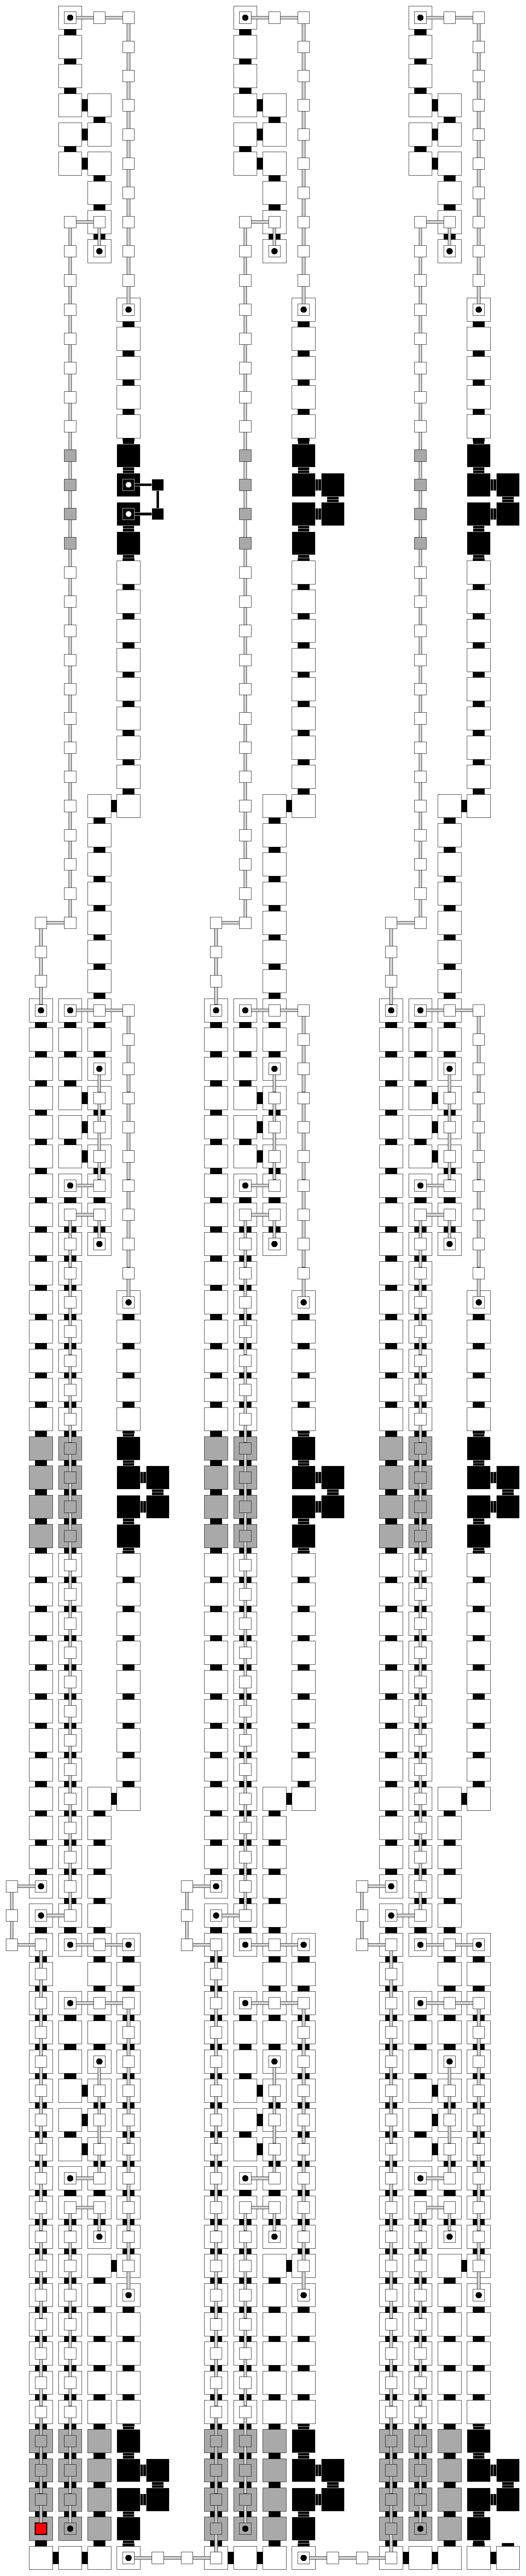
\includegraphics[width=0.3\textwidth]{seed/seed_overview_case3}
        \caption{\label{fig:initial_value_case3} Initial value case 3}
    \end{subfigure}%
    ~
    \begin{subfigure}[t]{0.3\textwidth}
        \centering
        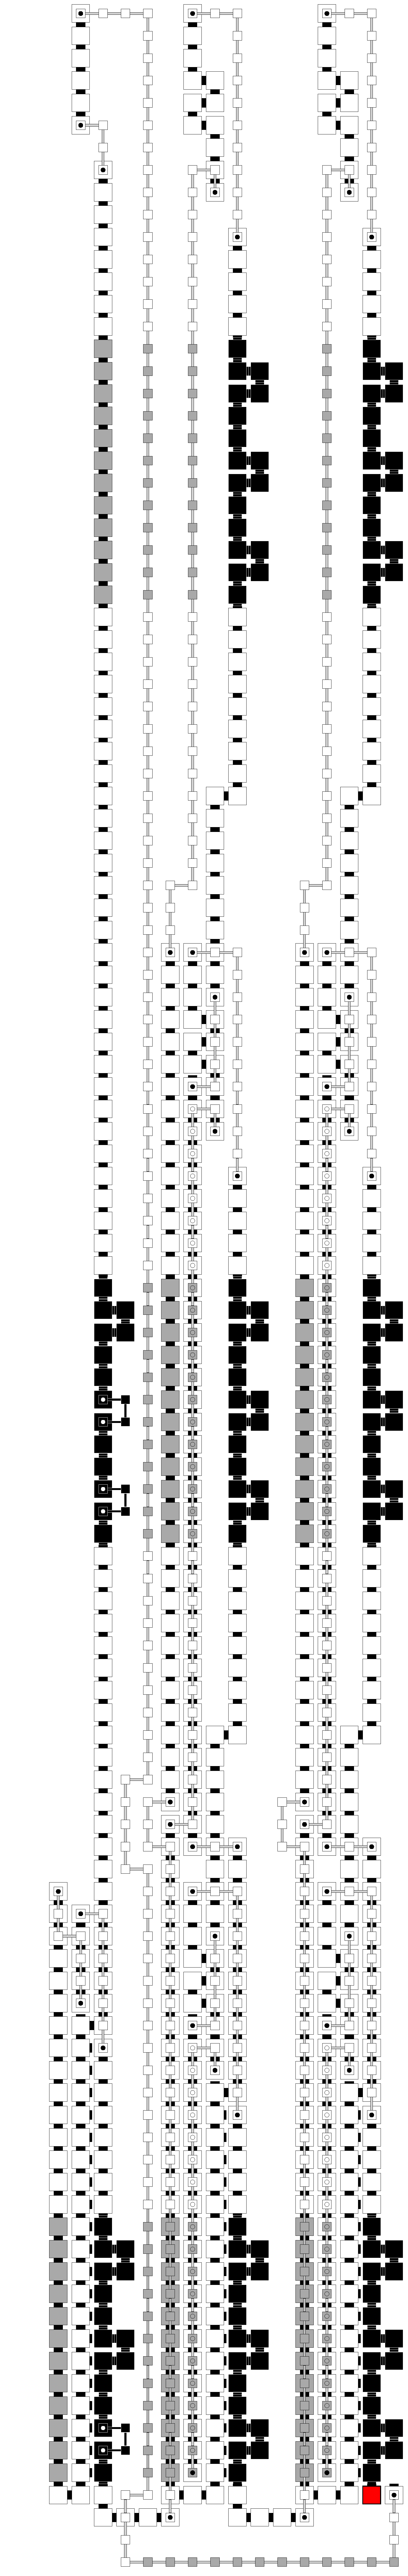
\includegraphics[width=0.3\textwidth]{seed/seed_overview_case2}
        \caption{\label{fig:initial_value_case2} Initial value case 2}
    \end{subfigure}%
    ~
    \begin{subfigure}[t]{0.3\textwidth}
        \centering
        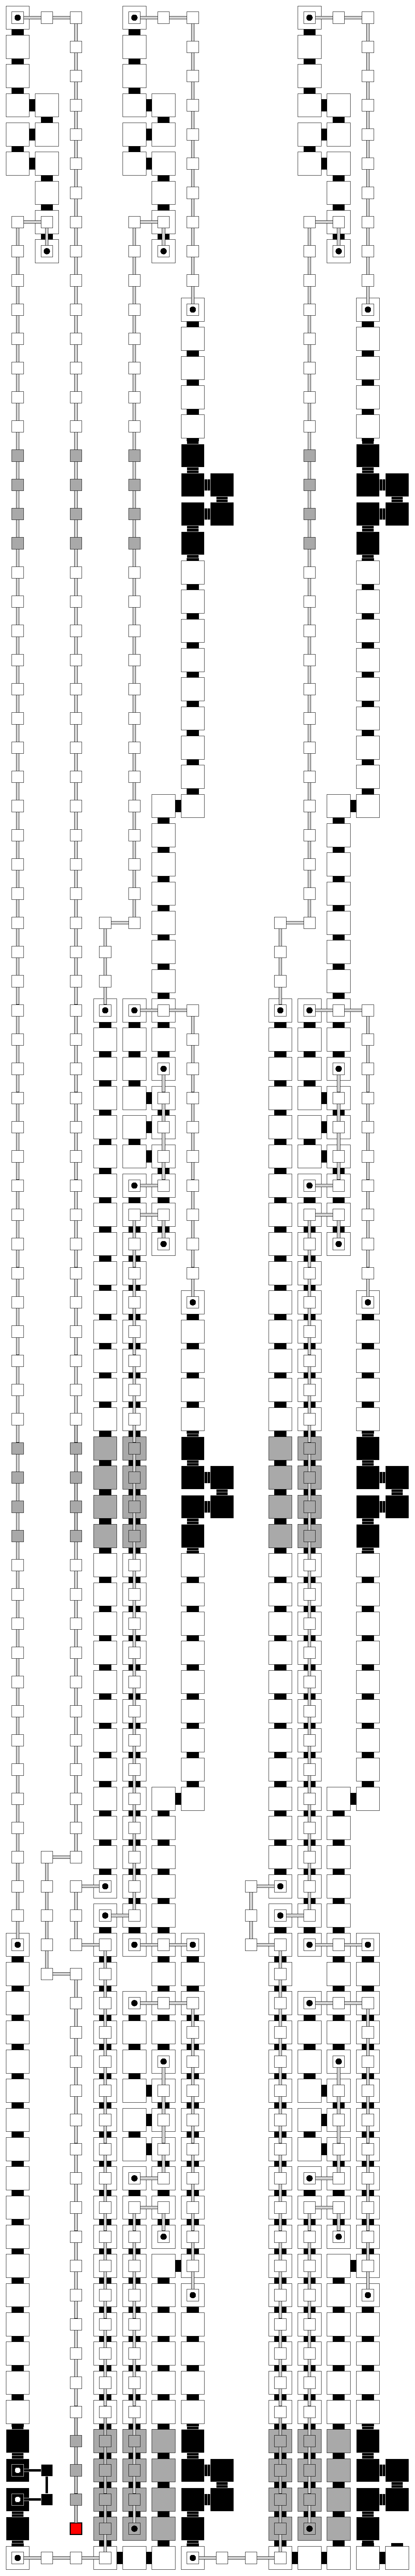
\includegraphics[width=0.3\textwidth]{seed/seed_overview_case1}
        \caption{\label{fig:initial_value_case1} Initial value case 1}
    \end{subfigure}%
    ~
\end{figure}
